% !TeX spellcheck = en_GB

% consider adding section just for bookmark purposes, not to be printed

% ******************************* %
% ******************************* %

\begin{frame}{Apple quality dataset}

\vspace*{-2.5em}\begin{columns}[T]
%\hspace*{2em}%
\begin{column}{0.5\textwidth}
Variables

%\begingroup\setlength{\tabcolsep}{0.25ex}
%\hspace*{-0.5em}\begin{tabular}{p{0.55\textwidth}p{0.5\textwidth}}
%\begin{itemize}
%	\item \texttt{Size}
%	\item \texttt{Weight}
%	\item \texttt{Sweetness}
%	\item \texttt{Crunchiness}
%\end{itemize}
%&
%\begin{itemize}
%	\item \texttt{Juiciness}
%	\item \texttt{Ripeness}
%	\item \texttt{Acidity}
%\end{itemize}
%\end{tabular}
%\endgroup

\begin{itemize}
	\item \texttt{Size}
	\item \texttt{Weight}
	\item \texttt{Sweetness}
	\item \texttt{Crunchiness}
	\item \texttt{Juiciness}
	\item \texttt{Ripeness}
	\item \texttt{Acidity}
\end{itemize}

\end{column}
\hspace*{-2em}%
\begin{column}{0.5\textwidth}
\alert{Binary classification} task% $\mathcal{Y}\in\set{0,1}$% (disease -- no disease)

Class distribution: 0.49 -- 0.51

\vspace{1em}Methods
\begin{itemize}
	\item $k\text{NN}$, Decision tree%, Logistic regression
	\item Random forest
	\item AdaBoost
	\item \alert{Super Learner}
\end{itemize}
\end{column}
\end{columns}

\end{frame}

% ******************************* %
% ******************************* %

\pdfbookmark[1]{Random Forest}{rf}

%\begin{frame}{Random forest}%{Random forest tuning}
%
%\begin{columns}[T]
%\hspace*{-3.4em}\begin{column}{0.5\textwidth}
%	\includegraphics[width=1.3\columnwidth]{biasvar-rf-apple}
%\end{column}
%\hspace*{-1.3em}\begin{column}{0.5\textwidth}
%	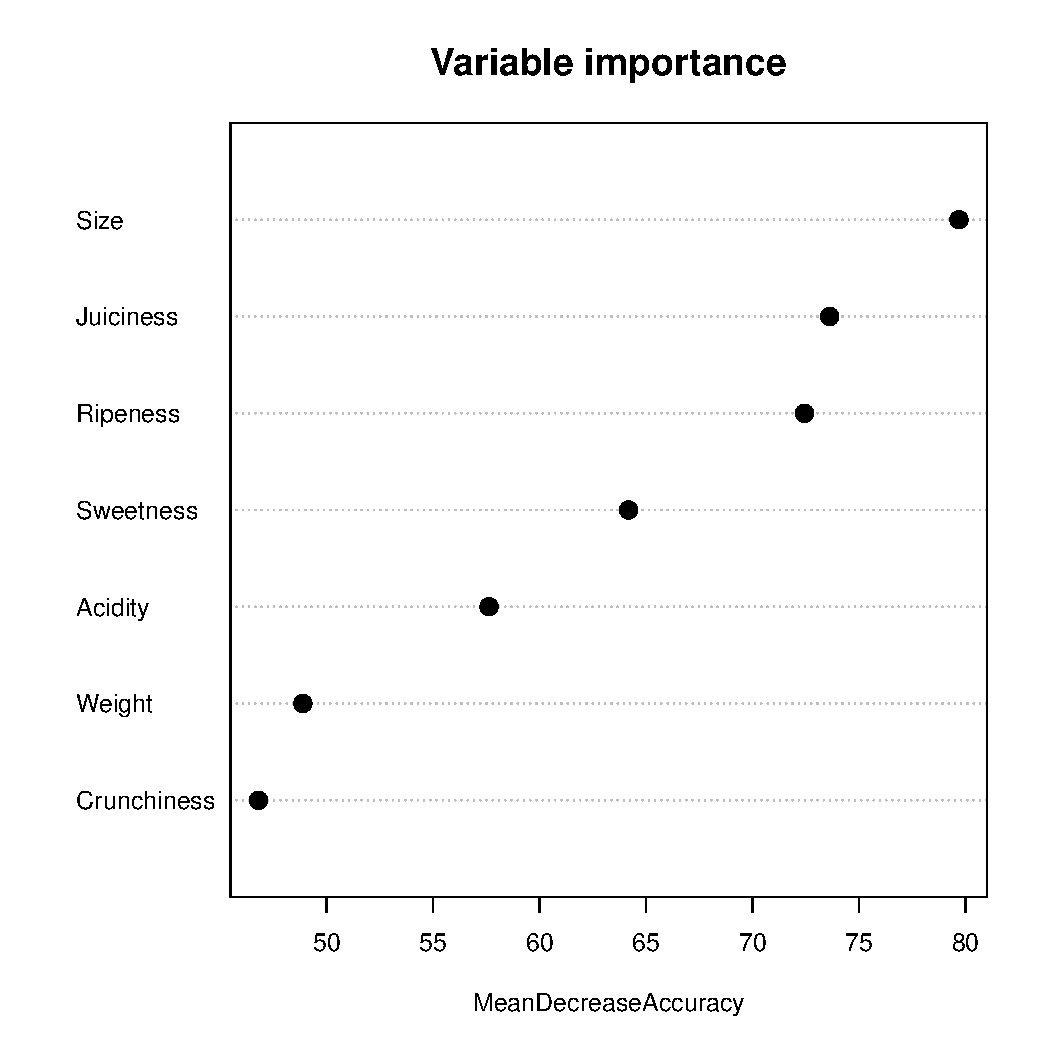
\includegraphics[width=1.3\columnwidth]{vip-rf-apple}
%\end{column}
%\end{columns}
%
%\begin{tikzpicture}
%	\node[rectangle,fill=red!20,font=\large,right] (mtry) at (0,0) {$\mathtt{mtry}=\lfloor\sqrt{p}\rfloor$};
%\end{tikzpicture}
%
%\end{frame}

% ------------------------------- %

\begin{frame}[fragile]{Random forest}

\begin{columns}[T]
\begin{column}{0.7\textwidth}
\begin{figure}
\centering
\hspace*{-7em}\vspace*{-0.5em}%
\begin{tikzpicture}
	%draw,ellipse,fill=red!20,minimum height=2em,text centered,font=\sffamily\small
	\tikzset{help lines/.append style=pink}
	%	\draw [help lines] (-1,-4) grid (7,2); \node[draw,circle,fill=red] at (0,0) {};
	
	\node[cloud3] (b1) at (0,0) {$\pi_1, m_1$};
	\node[cloud3] (b2) at ($(b1)+(1.8,0)$) {$\pi_2, m_2$};
	\node[cloud3] (B) at ($(b2)+(3,0)$) {$\pi_B, m_B$};
	\draw[-,dotted,very thick] (b1) to (b2);
	\draw[-,dotted,very thick] (b2) to (B);
	
	\node[] (T1) at ($(b1)+(0,-1.3)$) {$T_1$};
	\node[] (T2) at ($(b2)+(0,-1.3)$) {$T_2$};
	\node[] (TB) at ($(B)+(0,-1.3)$) {$T_B$};
	\draw[-stealth] ($(b1.south)+(0,-0.15)$) to (T1);
	\draw[-stealth] ($(b2.south)+(0,-0.15)$) to (T2);
	\draw[-stealth] ($(B.south)+(0,-0.15)$) to (TB);
	
	\begingroup\linespread{0.9}
	\node[font=\footnotesize,text width=4em,centered,text centered,inner sep=0pt] (m) at (3.3,0.7) {random predictors};
	\node[font=\footnotesize,text width=4em,centered,text centered,inner sep=0pt] (pi) at (3.1,-1.2) {random subsample};
	\endgroup
	\draw[-stealth] (m) to ($(b2.east)+(-0.2,0.1)$);
	\draw[-stealth] (pi) to ($(b2.south)+(-0.1,0.25)$);
	
	\node[rectangle,fill=mLightGreen!20,font=\large,right] (G) at (-0.8,-3) {$G(x)=\argmax_k\sum_{b=1}^B\mathbb{I}(T_b(x)=k)$};
	\node[rectangle,fill=red!20,font=\large,right] (mtry) at ($(G.west)+(0,-1)$) {$\mathtt{mtry}=\lfloor\sqrt{p}\rfloor$};
\end{tikzpicture}
\end{figure}
\end{column}
\hspace*{-6.5em}%
\begin{column}{0.4\textwidth}

\hspace*{-0.8em}\includegraphics[width=1.4\columnwidth]{../r-StatsLearn-Exam/src/plots/biasvar-rf-apple}

\end{column}
\end{columns}

\end{frame}

% ******************************* %
% ******************************* %

\pdfbookmark[1]{AdaBoost}{ada}

\begin{frame}[fragile]{AdaBoost algorithm}
% modello additivo perché in ogni albero c'è soltanto una variabile
\begin{columns}[T]
\begin{column}{0.48\textwidth}
\begin{figure}
\centering
\vspace*{-0.8em}\begin{tikzpicture}
	%draw,ellipse,fill=red!20,minimum height=2em,text centered,font=\sffamily\small
	\tikzset{help lines/.append style=pink}
%	\draw [help lines] (-2,-8) grid (3,1); \node[draw,circle,fill=red] at (0,0) {};
	
	\node[cloud2] (m1) at (0,0) {$w^{(1)}, \pi_1$};
	\node[cloud2] (m2) at (0,-1.25) {$w^{(2)}, \pi_2$};
	\node[cloud2] (M) at (0,-4.5) {$w^{(M)}, \pi_M$};
	\draw[-latex] (m1) to (m2);
	\draw[-,dotted,very thick] ($(m2.south) + (0,-0.15)$) to ($(M.north) + (0,+0.15)$);
	
	\node[right] (G1) at ($(m1)+(1.5,0)$) {$G_1, f_1, \alpha_1$};
	\node[right] (G2) at ($(m2)+(1.5,0)$) {$G_2, f_2, \alpha_2$};
	\node[right] (GM) at ($(M)+(1.5,0)$) {$G_M, f_M, \alpha_M$};
	\draw[-stealth] ($(m1.east) + (0.15,0)$) to (G1);
	\draw[-stealth] ($(m2.east) + (0.15,0)$) to (G2);
	%	\draw[-,dotted] (G2) to (GM);
	\draw[-stealth] ($(M.east) + (0.15,0)$) to (GM);
	
	%	\node[rectangle,fill=pink!80] (G) at (1.5,-6) {$G(x)=\sign\Bigl(\sum_{m=1}^M\beta_mG_m(x)\Bigr)$};
	\node[rectangle,fill=teal!20,font=\large,right] (G) at (-1,-5.55) {$f_m(x)=f_{m-1}(x)+\lambda\alpha_mG_m(x)$};
	\node[rectangle,fill=mLightGreen!20,font=\large,right] (L) at ($(G.west)+(0,-0.75)$) {$G(x)=\sign(f_M(x))$};
	\node[rectangle,fill=red!20,font=\large,right] (f) at ($(L.west)+(0,-0.75)$) {$L(y,f(x))=\exp(-yf(x))$};
	%	\draw[-stealth] (GM) to (G);
	
	\begingroup\linespread{0.9}
	\node[font=\footnotesize,text width=4em,centered,text centered,inner sep=0pt] (pi) at (2.8,-2.3) {random subsample};
	\node[font=\footnotesize,text width=4em,centered,text centered,inner sep=0pt] (w) at (1.1,-2.7) {sample weights};
	\endgroup
	\draw[-stealth] (pi) to ($(m2.east)+(-0.25,-0.1)$);
	\draw[-stealth] (w) to ($(m2.south)+(-0.25,0.25)$);
\end{tikzpicture}
\end{figure}
\end{column}
\begin{column}{0.48\textwidth}
%\vspace{0.7em}
%Journey to the final classifier:
%{\footnotesize\begin{itemize}
%\setlength{\itemsep}{-0.8ex}
%\item Linear combination of \alert{weak learners} (additive model)
%\item Adaptively build up complexity, through a prediction function
%\item Regularization with early stopping and shrinkage
%\item \alert{Re-weighting} of a bootstrapped fraction of the training data  % permette all'algoritmo di concentrarsi sugli esempi più difficili da classificare, quindi di questi esempi viene aumentato il peso
%\end{itemize}}

\vspace*{0.5em}Encoding $\mathcal{Y}\in\set{-1,1}$

\begin{lstlisting}
ada::ada(x, y,
  loss="exponential",
  type="discrete",
  iter£!$\,\alert{\leftarrow} M^\ast$!£, nu£!$\,\alert{\leftarrow}\lambda^\ast$!£,
  bag.frac£!$\,\alert{\leftarrow}\pi^\ast$!£,
  control=base.learner)
\end{lstlisting}

%\begin{columns}[T]
%\begin{column}{0.5\textwidth}
%\begin{tikzpicture}[]
%	\tikzset{help lines/.append style=pink}
%	%	\draw [help lines] (-2,-2) grid (2,1);
%	
%	\node[treenode] (root) at (0,0) {$-1$};
%	\node[treenode] (root-l) at (-120:1.35) {$-1$};
%	\node[treenode] (root-r) at (-60:1.35) {$1$};
%	
%	\draw[-] (root) -- node[font=\footnotesize,left] {$x_j<v$} (root-l);
%	\draw[-] (root) -- node[font=\footnotesize,right] {$x_j\geq v$} (root-r);
%\end{tikzpicture}
%\end{column}
%\hspace{-3em}\begin{column}{0.5\textwidth}
%\begin{tikzpicture}[]
%	\tikzset{help lines/.append style=pink}
%	%	\draw [help lines] (-3,-4) grid (3,1);
%	
%	\node[treenode] (root) at (0,0) {$-1$};
%	\node[treenode] (root-l) at (-130:1.4) {$-1$};
%	\node[treenode] (root-r) at (-50:1.4) {$1$};
%	\node[treenode] (ll) at ($(root-l)+(-110:1.25)$) {$1$};
%	\node[treenode] (lr) at ($(root-l)+(-70:1.25)$) {$-1$};
%	\node[treenode] (rl) at ($(root-r)+(-110:1.25)$) {$1$};
%	\node[treenode] (rr) at ($(root-r)+(-70:1.25)$) {$-1$};
%	
%	\draw[-] (root) -- (root-l);
%	\draw[-] (root) -- (root-r);
%	\draw[-] (root-l) -- (ll); \draw[-] (root-l) -- (lr);
%	\draw[-] (root-r) -- (rl); \draw[-] (root-r) -- (rr);
%\end{tikzpicture}
%\end{column}
%\end{columns}

\vspace{1.5em}\begin{center}%
\begin{tikzpicture}[]
	\tikzset{help lines/.append style=pink}
%	\draw [help lines] (-2,-2) grid (2,1);
	
	\node[treenode] (root) at (0,0) {$-1$};
	\node[treenode] (root-l) at (-120:1.35) {$-1$};
	\node[treenode] (root-r) at (-60:1.35) {$1$};
	
	\draw[-] (root) -- node[font=\scriptsize,left] {$x_j<v$} (root-l);
	\draw[-] (root) -- node[font=\scriptsize,right] {$x_j\geq v$} (root-r);

	\draw[|-|] ($(root)+(1.65,0)$) -- node[right,font=\footnotesize] {$d=1$} ++ (0,-{1.35*cos(30)});
\end{tikzpicture}%
\end{center}

\end{column}
\end{columns}

\end{frame}

% ------------------------------- %

%\begin{frame}{AdaBoost tuning}
%
%\begin{columns}[T]
%\hspace*{-2.4em}\begin{column}{0.5\textwidth}
%	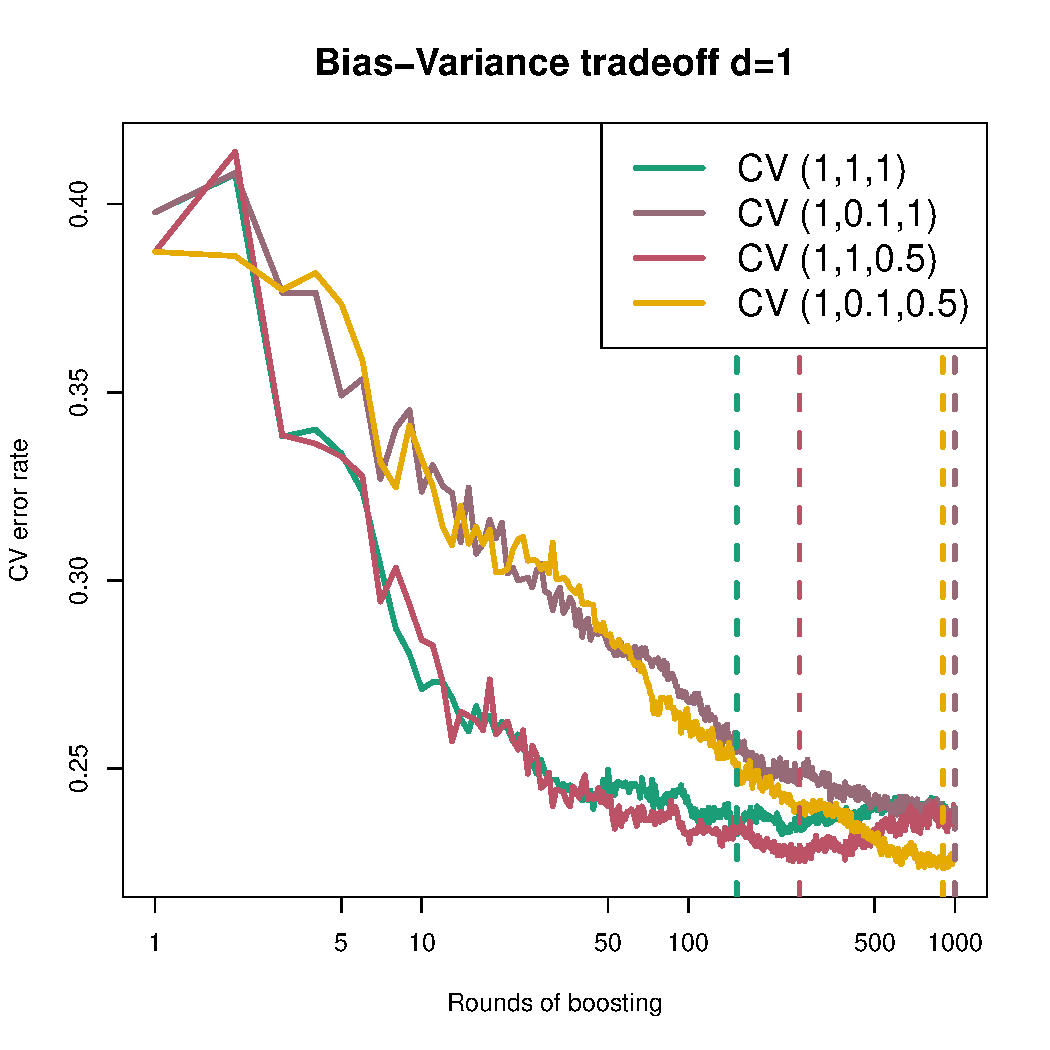
\includegraphics[width=1.23\columnwidth]{biasvar-ada1-apple}
%\end{column}
%\begin{column}{0.5\textwidth}
%	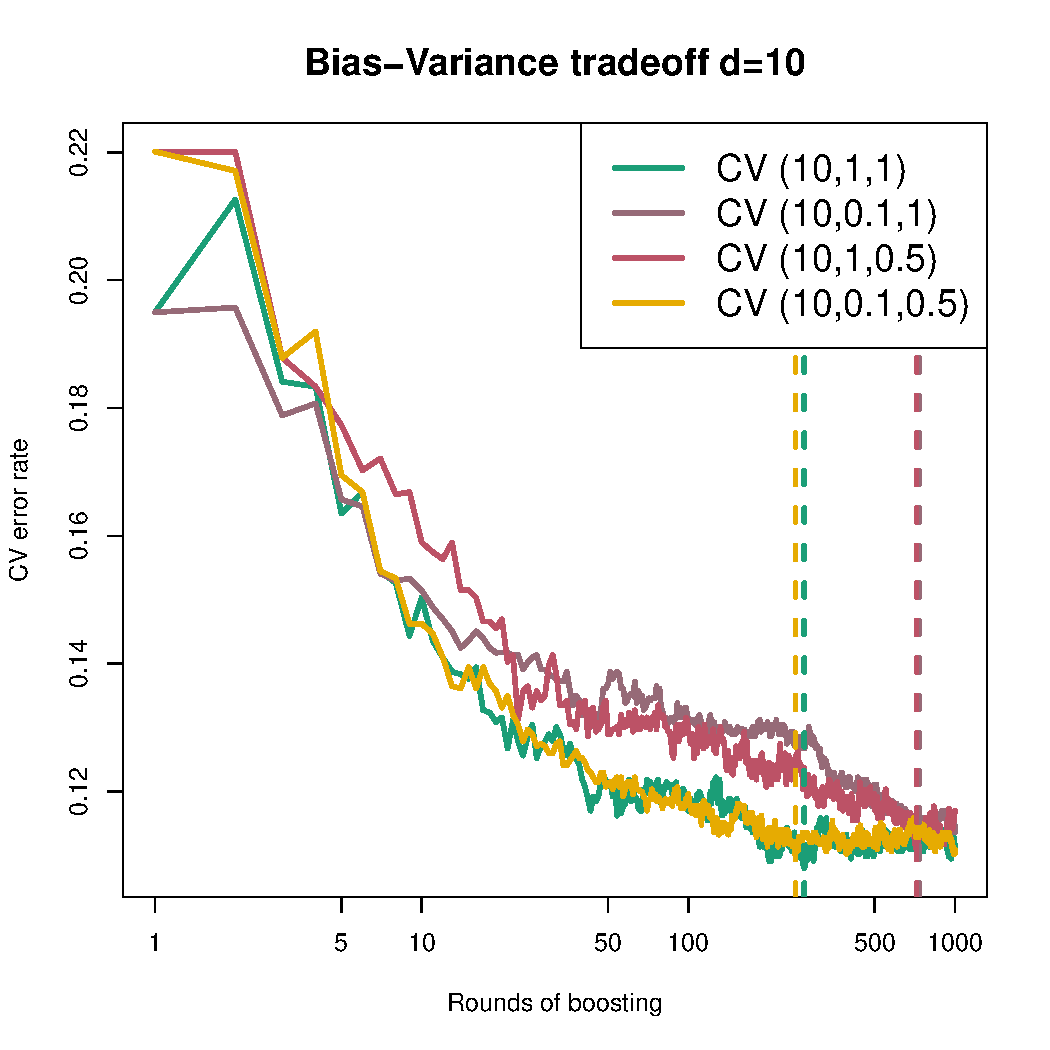
\includegraphics[width=1.23\columnwidth]{biasvar-ada2-apple}
%\end{column}
%\end{columns}
%
%\end{frame}

\begin{frame}{AdaBoost tuning}

% soltanto il CV error per questioni di spazio e comunque perché il training va diretto a 0 senza troppi complimenti

% per d>1 si perde la proprietà di additività del modello
% il vantaggio rispetto alla random forest lo perde un po'

\begin{columns}[T]
\hspace*{-2.6em}\begin{column}{0.5\textwidth}
	\begin{tikzpicture}
		\tikzset{help lines/.append style=pink}
%		\draw[help lines] (0,0) grid (6,6); \node[draw,circle,fill=red] at (0,0) {};
		\node[immagine] at (0,0) {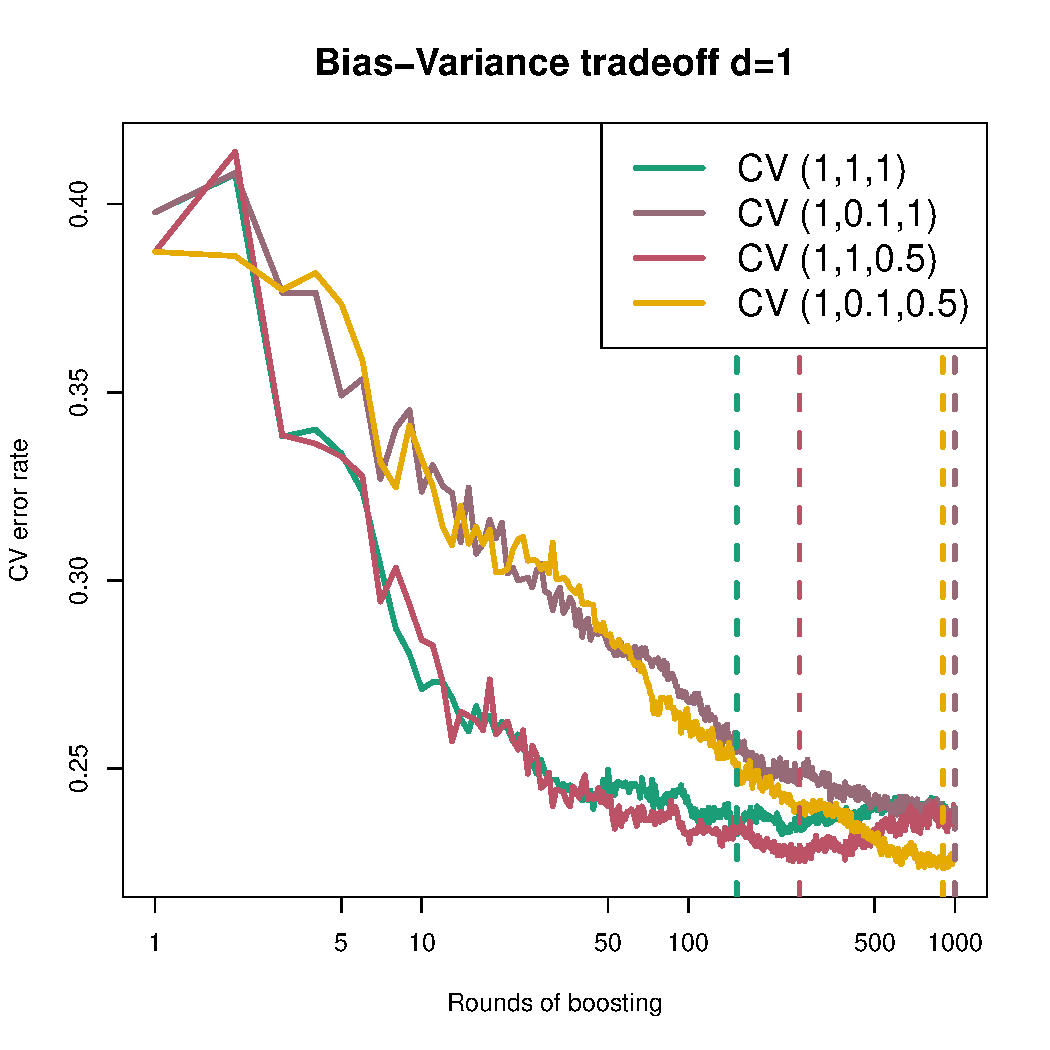
\includegraphics[width=1.25\columnwidth]{biasvar-ada1-apple}};
		\node[draw,rectangle,inner xsep=1.05cm,inner ysep=0.9ex,red,very thick] at (5.25,4.8) {};
	\end{tikzpicture}
\end{column}
\begin{column}{0.5\textwidth}
	\begin{tikzpicture}
		\tikzset{help lines/.append style=pink}
%		\draw[help lines] (0,0) grid (6,6); \node[draw,circle,fill=red] at (0,0) {};
		\node[immagine] at (0,0) {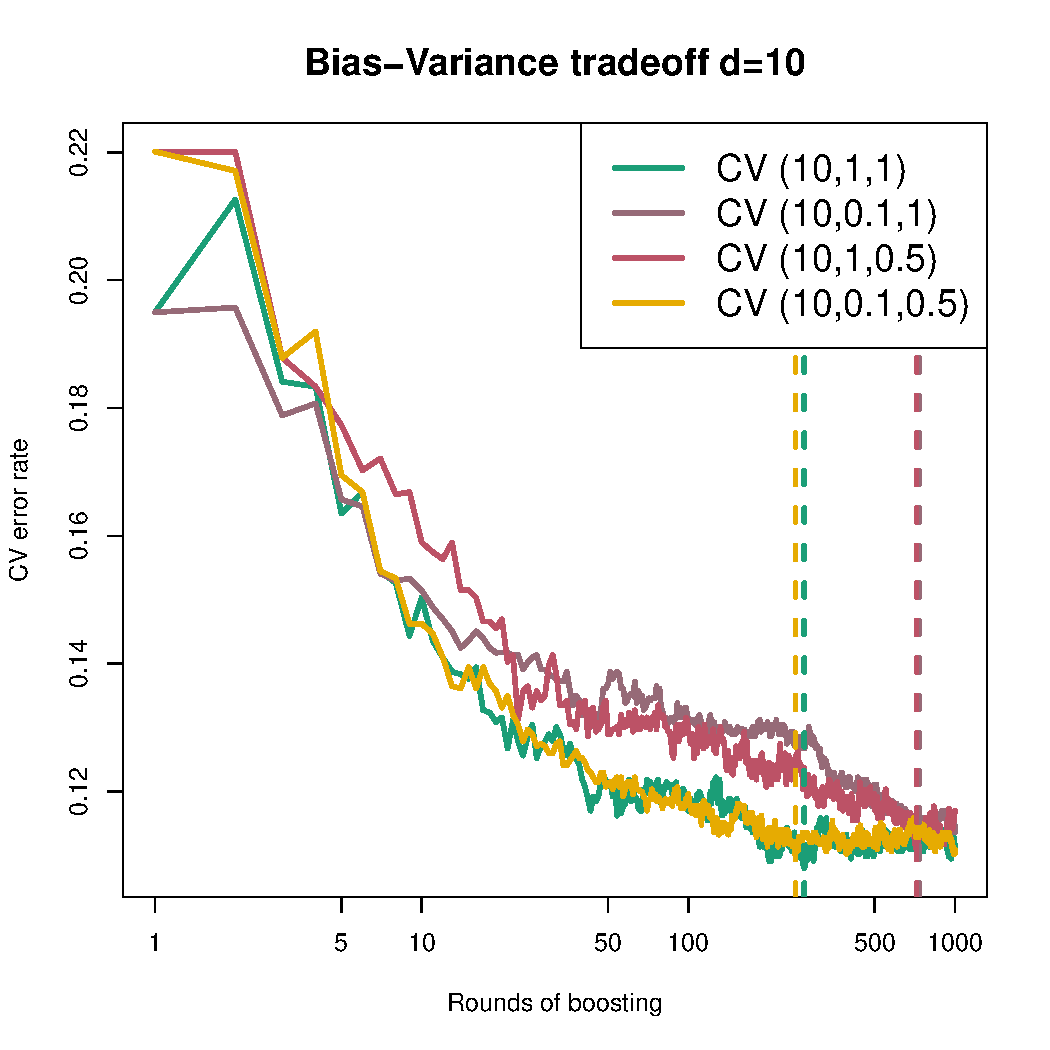
\includegraphics[width=1.25\columnwidth]{biasvar-ada2-apple}};
		\node[draw,rectangle,inner xsep=1.05cm,inner ysep=0.9ex,red,very thick] at (5.25,4.8) {};
	\end{tikzpicture}
\end{column}
\end{columns}

\end{frame}

% ------------------------------- %

%\begin{frame}{AdaBoost variable importance}
%
%% la scale sull'ascisse va bene?
%
%% mi interessava riproporre questa analisi perché volevo indagare sulla differente selezione delle variabili da parte dei due modelli
%
%\begin{columns}[T]
%\hspace*{-3.9em}%
%\begin{column}{0.5\textwidth}
%	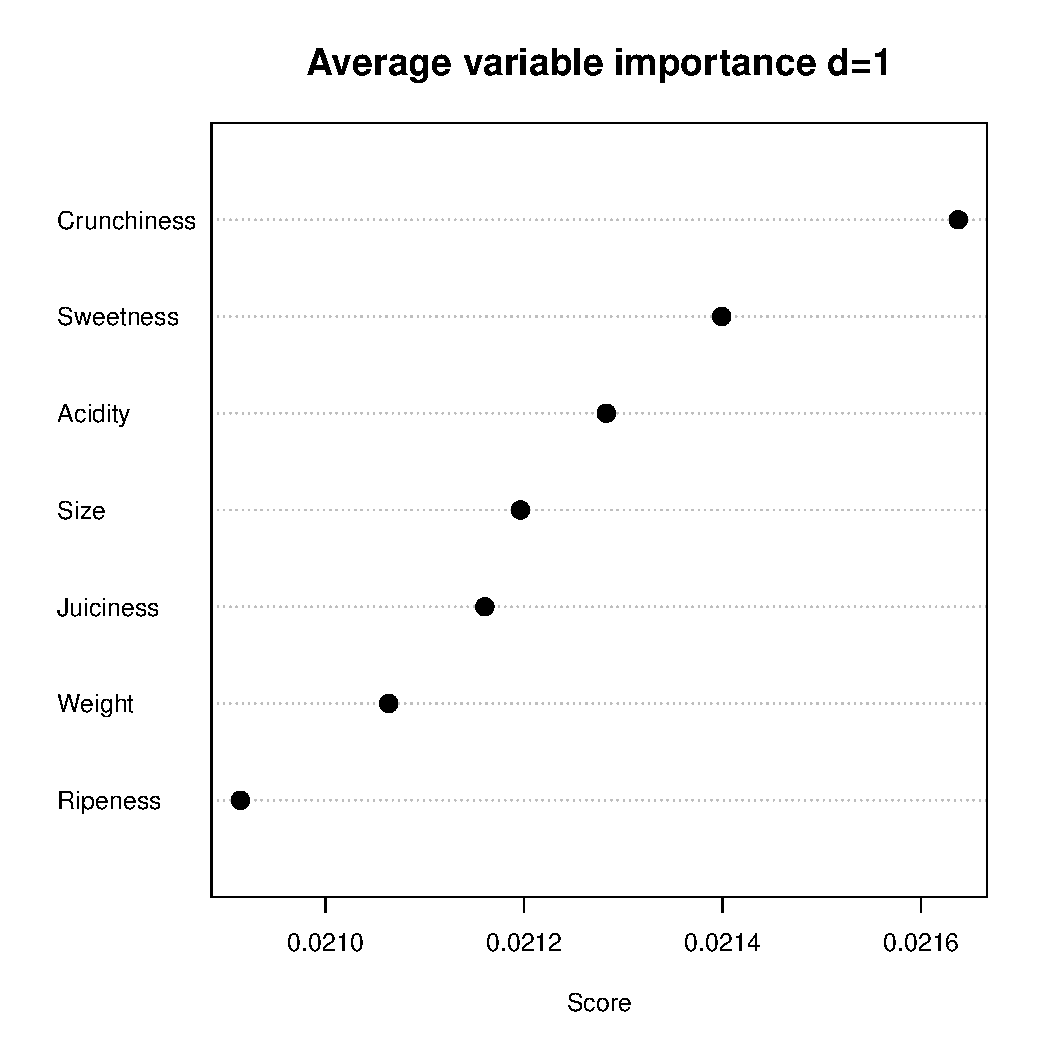
\includegraphics[width=1.25\columnwidth]{vip-ada1-apple}
%\end{column}
%\hspace*{-1em}%
%\begin{column}{0.5\textwidth}
%	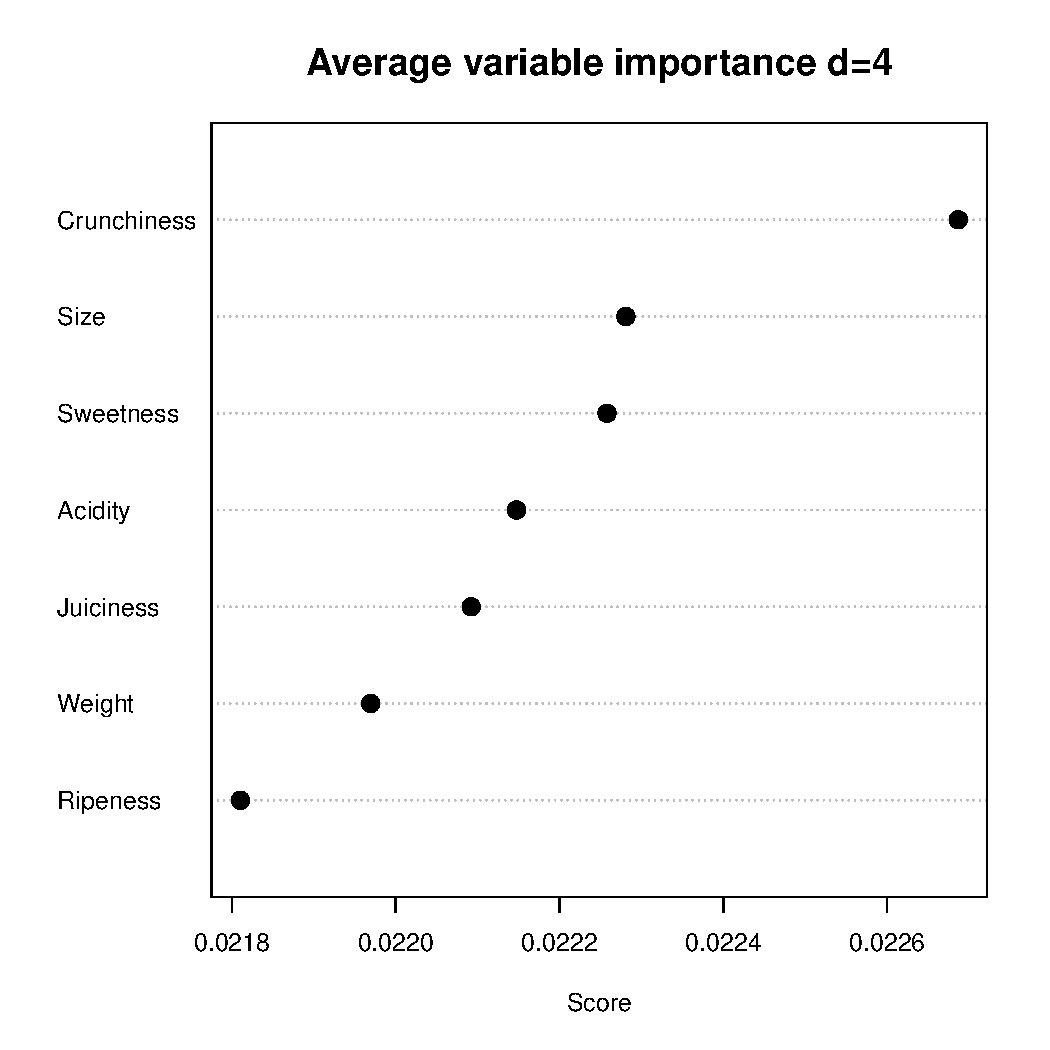
\includegraphics[width=1.25\columnwidth]{vip-ada2-apple}
%\end{column}
%\end{columns}
%
%\end{frame}

% ******************************* %
% ******************************* %

\begin{frame}{Variable importance comparison}

% random forest dà più importanza alla succosità e allo stato di maturazione
% adaboost dà più importanza alla croccantezza, caratteristica che una mela marcia perde, come la dolcezza

\begin{columns}[T]
\hspace*{-4.2em}%
\begin{column}{0.3\textwidth}
	\begin{tikzpicture}
		\tikzset{help lines/.append style=pink}
%		\draw[help lines] (0,0) grid (5,5); \node[draw,circle,fill=red] at (0,0) {};
		\node[immagine] (img) at (0,0) {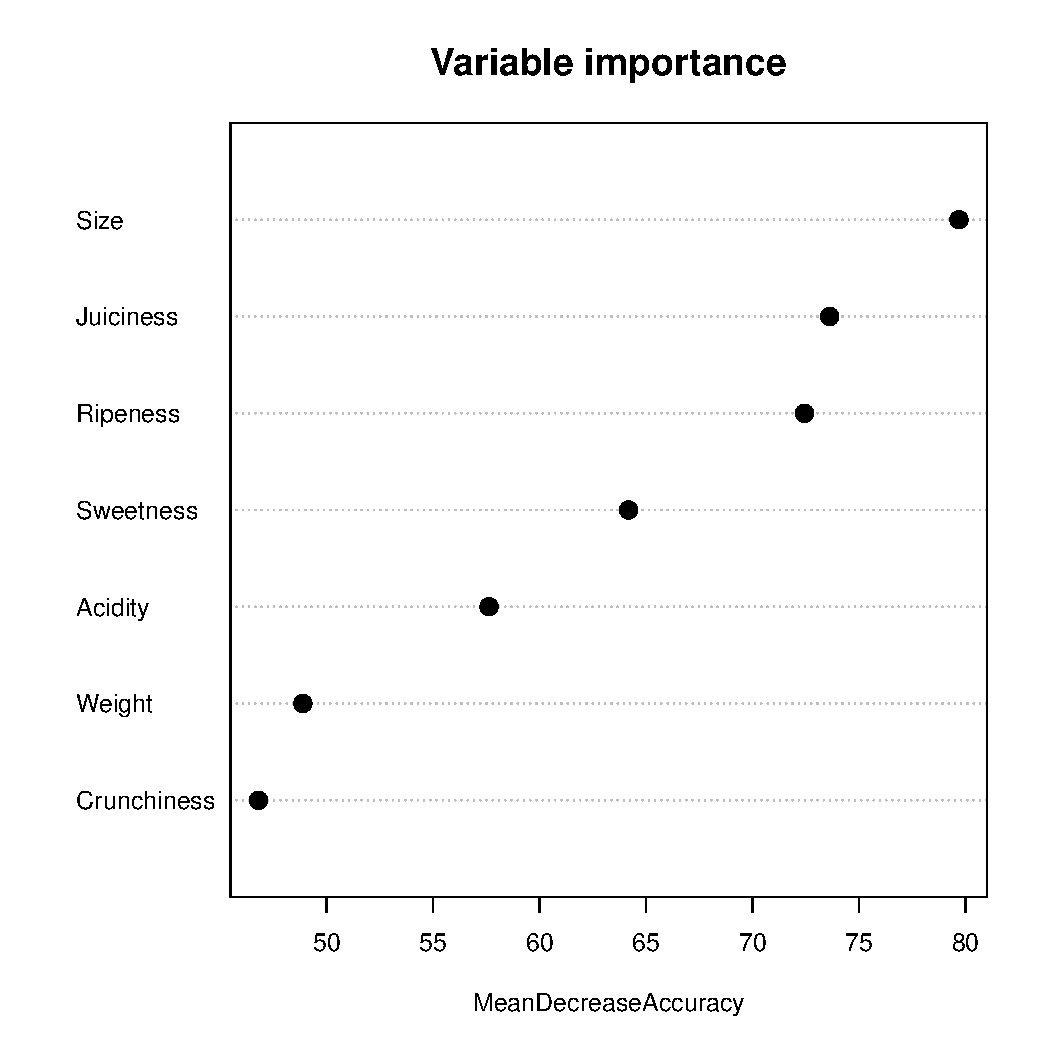
\includegraphics[width=1.47\columnwidth]{vip-rf-apple}};
		\node[font=\small] at ($(img)+(0.3,3)$) {Random Forest};
		\node[draw,rectangle,inner xsep=0.35cm,inner ysep=0.7ex,mLightBrown,thick] at (0.66,1.13) {};
		\node[draw,rectangle,inner xsep=0.28cm,inner ysep=0.7ex,mLightGreen,thick] at (0.59,2.89) {};
	\end{tikzpicture}
\end{column}
\hspace*{-0.7em}%
\begin{column}{0.3\textwidth}
	\begin{tikzpicture}
		\tikzset{help lines/.append style=pink}
%		\draw[help lines] (0,0) grid (5,5); \node[draw,circle,fill=red] at (0,0) {};
		\node[immagine] at (0,0) {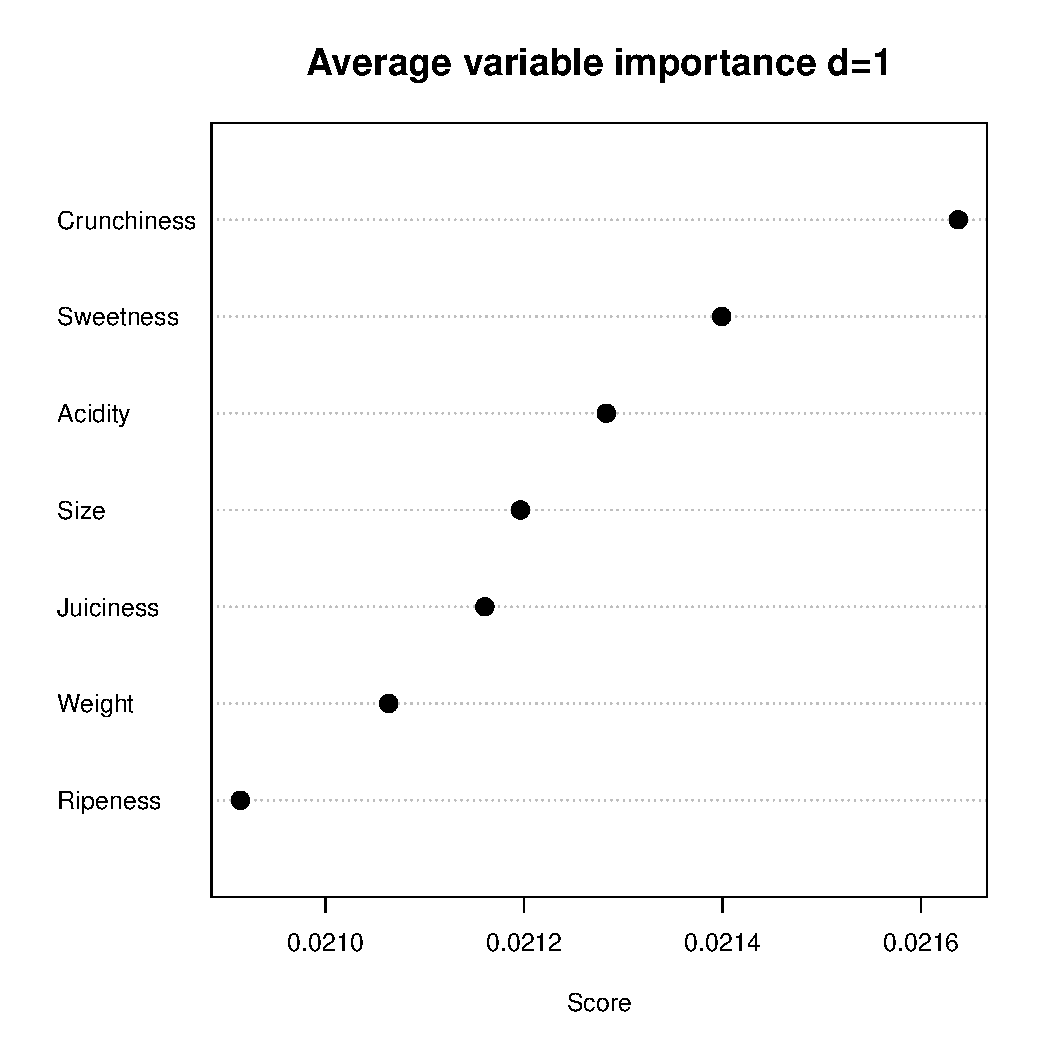
\includegraphics[width=1.47\columnwidth]{vip-ada1-apple}};
		\node[font=\small] at ($(img)+(0.3,3)$) {$\text{AdaBoost}_{d=1}$};
		\node[draw,rectangle,inner xsep=0.28cm,inner ysep=0.7ex,mLightGreen,thick] at (0.505,1.135) {};
		\node[draw,rectangle,inner xsep=0.35cm,inner ysep=0.7ex,mLightBrown,thick] at (0.575,3.77) {};
	\end{tikzpicture}
\end{column}
\hspace*{-0.7em}%
\begin{column}{0.3\textwidth}
	\begin{tikzpicture}
		\node[immagine] at (0,0) {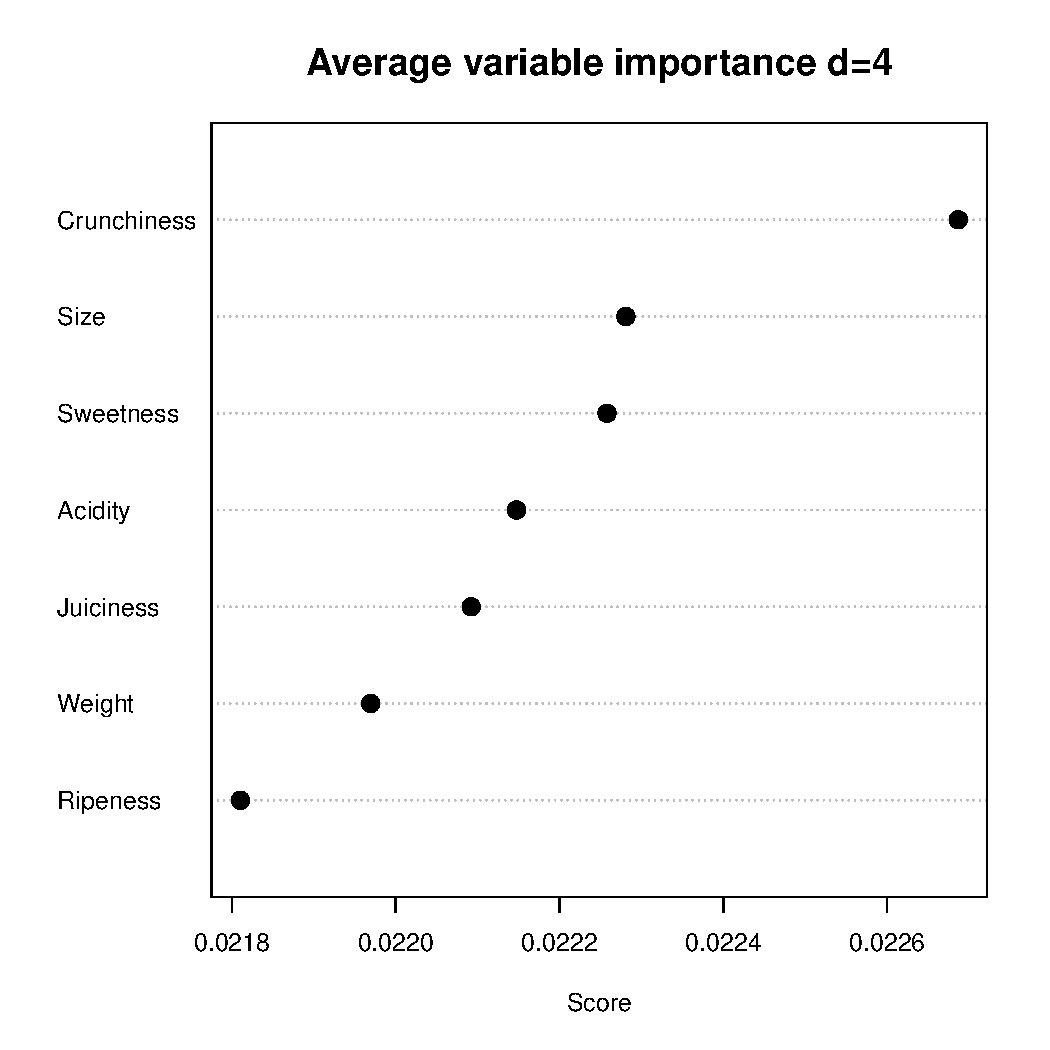
\includegraphics[width=1.47\columnwidth]{vip-ada2-apple}};
		\node[font=\small] at ($(img)+(0.3,3)$) {$\text{AdaBoost}_{d=4}$};
		\node[draw,rectangle,inner xsep=0.28cm,inner ysep=0.7ex,mLightGreen,thick] at (0.505,1.135) {};
		\node[draw,rectangle,inner xsep=0.35cm,inner ysep=0.7ex,mLightBrown,thick] at (0.575,3.77) {};
	\end{tikzpicture}
\end{column}
\end{columns}

\end{frame}


